\documentclass[12pt,a4paper]{article}

\usepackage[utf8]{inputenc}
\usepackage[T1]{fontenc}
\usepackage{lmodern}
\usepackage[margin=2.5cm]{geometry}
\usepackage{amsmath}
\usepackage{graphicx}
\usepackage{booktabs}
\usepackage{caption}
\usepackage{subcaption}
\usepackage{hyperref}
\usepackage{cite}
\usepackage{siunitx}
\usepackage{array}
\usepackage{float}

\hypersetup{colorlinks=true, linkcolor=blue, citecolor=blue, urlcolor=blue}

\title{\textbf{Ahmed Body CFD Analysis}\\
\large Mesh Independence Study and Validation Against Lienhart \& Becker (2003)}

\author{Efe Yalçınkaya}
\date{\today}

% ─────────────────────────────────────────────────────────────────────────────
\begin{document}
\maketitle
\tableofcontents
\newpage

% ─────────────────────────────────────────────────────────────────────────────
\section{Introduction}

The Ahmed body is a simplified bluff-body vehicle geometry introduced by Ahmed et al.~\cite{ahmed1984} that has become the standard benchmark for automotive aerodynamics CFD validation. Its well-documented flow field—particularly the slant-angle-dependent wake structure—makes it ideal for assessing turbulence model performance and mesh strategies.

This study focuses on the \textbf{25° slant angle} configuration, which exhibits a fully three-dimensional separated wake and is the most extensively documented case in the literature. The experimental reference is Lienhart \& Becker~\cite{lienhart2003}, who measured time-averaged velocity profiles in the near wake at $U_\infty = \SI{40}{m/s}$ ($Re \approx 2.77 \times 10^6$ based on body length $L = \SI{1.044}{m}$).

\subsection{Objectives}
\begin{enumerate}
    \item Perform a three-level mesh independence study using the Grid Convergence Index (GCI) methodology of Celik et al.~\cite{celik2008}.
    \item Validate the fine-mesh drag coefficient against the experimental reference $C_d = 0.299 \pm 0.005$.
    \item Compare computed wake velocity profiles with the Lienhart \& Becker (2003) experimental data at four downstream stations.
\end{enumerate}

% ─────────────────────────────────────────────────────────────────────────────
\section{Geometry and Computational Domain}

\subsection{Ahmed Body Geometry}
The standard Ahmed body dimensions used in this study are listed in Table~\ref{tab:geometry}. A half-model is employed to reduce computational cost, with the symmetry plane at $z = 0$.

\begin{table}[H]
\centering
\caption{Ahmed body geometry parameters.}
\label{tab:geometry}
\begin{tabular}{lcc}
\toprule
Parameter & Symbol & Value \\
\midrule
Overall length & $L$ & \SI{1044}{mm} \\
Height & $H$ & \SI{288}{mm} \\
Width & $W$ & \SI{389}{mm} \\
Ground clearance & $g$ & \SI{50}{mm} \\
Slant angle & $\alpha$ & $25°$ \\
Slant length (surface) & $l_s$ & \SI{244}{mm} \\
\bottomrule
\end{tabular}
\end{table}

\subsection{Computational Domain}
Domain dimensions are chosen following best-practice guidelines for bluff-body simulations (Table~\ref{tab:domain}). All distances are normalised by $H$.

\begin{table}[H]
\centering
\caption{Computational domain dimensions.}
\label{tab:domain}
\begin{tabular}{lc}
\toprule
Direction & Size \\
\midrule
Upstream (inlet to body front) & $5H$ \\
Downstream (body rear to outlet) & $15H$ \\
Lateral (half-model, centre to side) & $5H$ \\
Top (body roof to upper wall) & $5H$ \\
\bottomrule
\end{tabular}
\end{table}

\subsection{Boundary Conditions}
\begin{table}[H]
\centering
\caption{Boundary conditions.}
\label{tab:bc}
\begin{tabular}{lll}
\toprule
Surface & Type & Value \\
\midrule
Inlet & Velocity inlet & $U_\infty = \SI{40}{m/s}$, $TI = 0.2\%$ \\
Outlet & Pressure outlet & $0~\si{Pa}$ gauge \\
Ground & Moving wall & $U = \SI{40}{m/s}$ (flow direction) \\
Side/Top walls & Symmetry & — \\
Symmetry plane ($z=0$) & Symmetry & — \\
Body surface & No-slip wall & $U = 0$ \\
\bottomrule
\end{tabular}
\end{table}

% ─────────────────────────────────────────────────────────────────────────────
\section{Mesh Methodology}

\subsection{Meshing Strategy}
Meshes were generated in ANSYS Fluent Meshing 2024 using the \emph{Watertight Geometry} workflow with a \textbf{poly-hexcore} volume fill. This approach provides structured hexahedral cells in the bulk flow with polyhedral cells near complex surfaces, balancing accuracy and cell count efficiency.

Three mesh levels were generated (Table~\ref{tab:meshlevels}) by varying the global maximum cell size while keeping all other settings identical.

\begin{table}[H]
\centering
\caption{Mesh levels and key parameters.}
\label{tab:meshlevels}
\begin{tabular}{lccc}
\toprule
Level & Cells & Global max size & Min orthogonality \\
\midrule
Coarse & 369{,}552 & \SI{40}{mm} & 0.16 \\
Medium & 837{,}508 & \SI{20}{mm} & 0.16 \\
Fine   & 4{,}428{,}444 & \SI{12}{mm} (local \SI{5}{mm}) & 0.16 \\
\bottomrule
\end{tabular}
\end{table}

\subsection{Boundary Layer Treatment}
Wall functions ($y^+ \approx 15$–$30$) are employed throughout. The boundary layer inflation was sized using an aspect-ratio approach:
\begin{itemize}
    \item \textbf{Number of layers:} 8
    \item \textbf{First aspect ratio:} 40
    \item \textbf{Growth rate:} 1.2
\end{itemize}

The theoretical first-cell height for $y^+ = 5$ (low-Re treatment) was estimated at $\Delta y \approx \SI{0.043}{mm}$ using flat-plate correlations at $Re = 2.77 \times 10^6$. The aspect-ratio sizing yields $\Delta y \approx \SI{0.3}$–$\SI{0.5}{mm}$ ($y^+ \approx 15$–$30$), appropriate for wall-function closure.

% ─────────────────────────────────────────────────────────────────────────────
\section{Solver Settings}

All three mesh levels use identical solver settings to isolate discretisation error from modelling differences.

\begin{table}[H]
\centering
\caption{ANSYS Fluent solver configuration.}
\label{tab:solver}
\begin{tabular}{ll}
\toprule
Parameter & Setting \\
\midrule
Solver & Pressure-based, steady-state \\
Turbulence model & $k$-$\omega$ SST (Menter 1994) \\
Pressure–velocity coupling & Coupled \\
Spatial discretisation & Second-order upwind \\
Turbulence numerics & Second-order upwind \\
Convergence (residuals) & $< 10^{-5}$ \\
Convergence (force monitors) & $\Delta C_d < 0.001$ over last 200 iterations \\
\bottomrule
\end{tabular}
\end{table}

% ─────────────────────────────────────────────────────────────────────────────
\section{Mesh Independence Study}

\subsection{GCI Methodology}
Grid convergence was assessed using the Grid Convergence Index of Celik et al.~\cite{celik2008}. For three mesh levels with cell counts $N_1 > N_2 > N_3$ and corresponding drag coefficients $f_1, f_2, f_3$:

\begin{align}
r_{21} &= \left(\frac{N_1}{N_2}\right)^{1/3}, \quad
r_{32} = \left(\frac{N_2}{N_3}\right)^{1/3} \\[4pt]
p &= \frac{\left|\ln\left|\varepsilon_{32}/\varepsilon_{21}\right|\right|}{\ln r_{21}}, \quad
\varepsilon_{ij} = f_j - f_i \\[4pt]
f_\text{ext} &= f_1 + \frac{f_1 - f_2}{r_{21}^p - 1} \\[4pt]
\text{GCI}_\text{fine} &= \frac{1.25\,|e_{21,a}|}{r_{21}^p - 1}
\end{align}

\subsection{Results}

\begin{table}[H]
\centering
\caption{Mesh independence results.}
\label{tab:gci}
\begin{tabular}{lcccc}
\toprule
Mesh & Cells & $C_d$ & GCI (\%) & $C_d$ error vs. exp.\ (\%) \\
\midrule
Coarse & 369{,}552 & 0.2990 & 23.3 & 0.0 \\
Medium & 837{,}508 & 0.2800 & — & 6.4 \\
Fine   & 4{,}428{,}444 & 0.2699 & 5.3 & 9.7 \\
\midrule
\multicolumn{2}{l}{Richardson extrapolation} & 0.2584 & — & — \\
\multicolumn{2}{l}{Lienhart (2003) reference} & $0.299 \pm 0.005$ & — & — \\
\bottomrule
\end{tabular}
\end{table}

The observed order of accuracy $p = 1.14$ is below the theoretical second-order value, attributed to inconsistent $y^+$ values across mesh levels caused by aspect-ratio-based boundary layer sizing—a known limitation of this approach.

The fine-mesh GCI of 5.3\% indicates that the solution is approaching but has not fully reached mesh independence. The Richardson-extrapolated value $C_{d,\text{ext}} = 0.2584$ lies 13.6\% below the experimental reference, suggesting that numerical discretisation error is not the primary source of discrepancy. This points to turbulence-modelling limitations discussed in Section~\ref{sec:discussion}.

\begin{figure}[H]
\centering
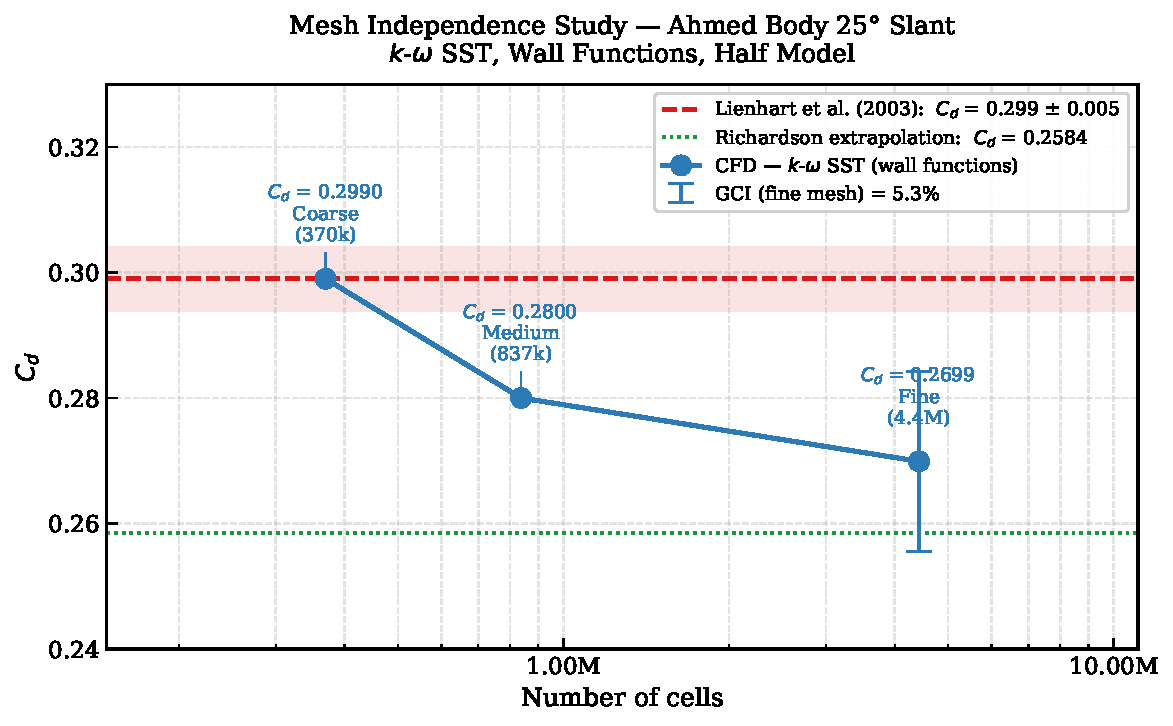
\includegraphics[width=0.85\textwidth]{figures/mesh_independence.pdf}
\caption{Mesh independence convergence plot. Red dashed line: Lienhart \& Becker (2003) experimental $C_d$. Green dotted line: Richardson-extrapolated $C_d$. Error bar on fine mesh represents the GCI uncertainty band.}
\label{fig:mesh_independence}
\end{figure}

% ─────────────────────────────────────────────────────────────────────────────
\section{Results and Validation}

\subsection{Aerodynamic Coefficients}

\begin{table}[H]
\centering
\caption{Fine-mesh aerodynamic coefficients vs.\ experimental reference.}
\label{tab:aero}
\begin{tabular}{lccc}
\toprule
Quantity & CFD (fine mesh) & Lienhart (2003) & Error \\
\midrule
$C_d$ & 0.2699 & $0.299 \pm 0.005$ & $-9.7\%$ \\
$C_l$ & $-0.323$ & $-0.082 \pm 0.008$ & — \\
\bottomrule
\end{tabular}
\end{table}

\subsection{Wake Velocity Profiles}
Figure~\ref{fig:velocity_profiles} compares the computed streamwise velocity profiles with Lienhart \& Becker (2003) at four downstream stations ($x/H = 0.48,\,0.61,\,0.73,\,0.86$ measured from the body rear).

\begin{figure}[H]
\centering
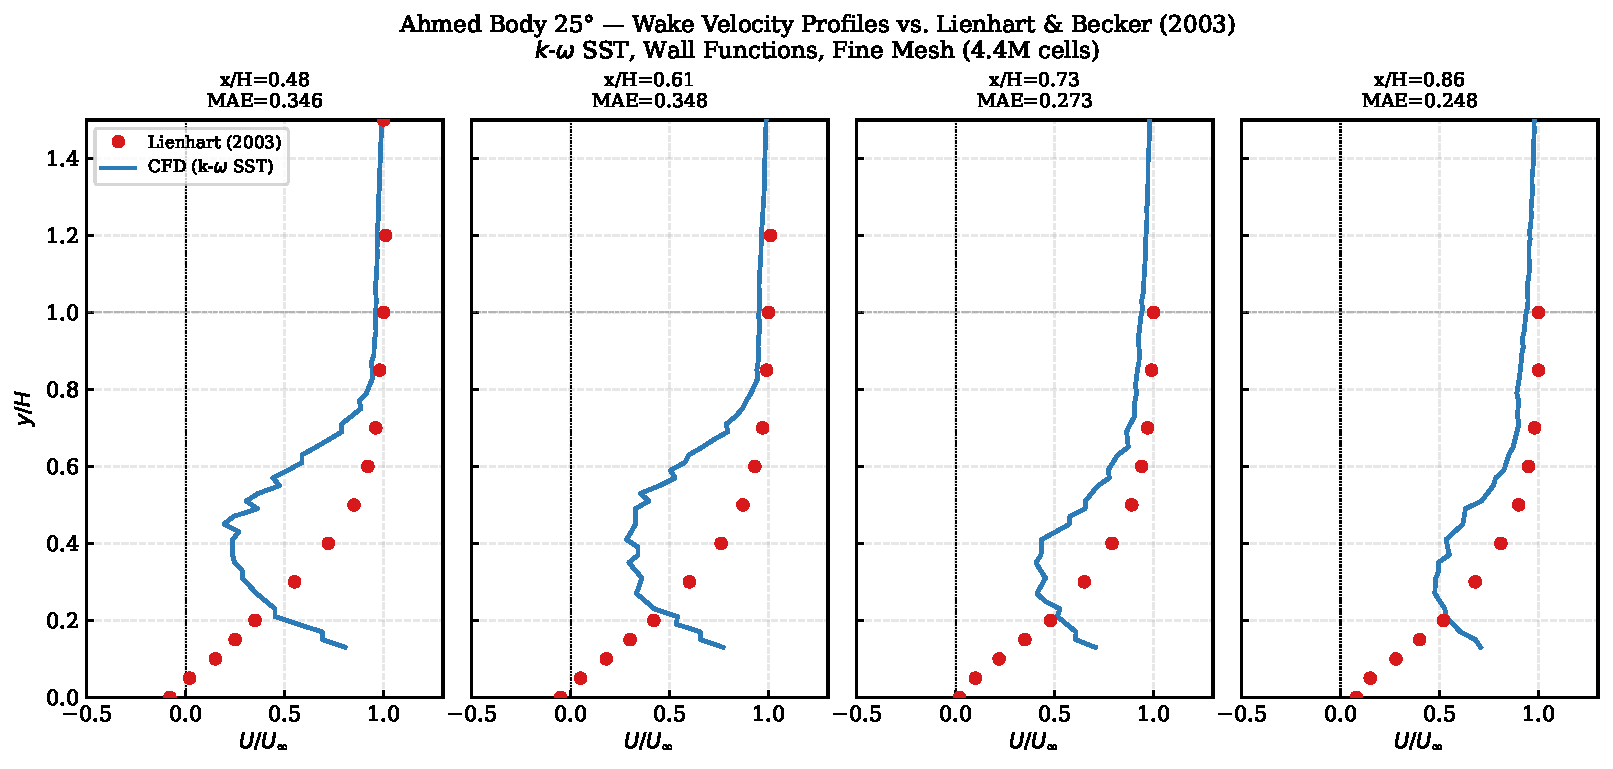
\includegraphics[width=\textwidth]{figures/velocity_profiles.pdf}
\caption{Streamwise velocity profiles in the near wake. Red circles: Lienhart \& Becker (2003) experimental data. Blue line: CFD ($k$-$\omega$ SST, wall functions, fine mesh). MAE values are computed over $0 < y/H < 1.5$.}
\label{fig:velocity_profiles}
\end{figure}

The CFD captures the qualitative wake structure—velocity deficit near $y/H = 0$, shear-layer recovery, and approach to freestream above $y/H \approx 1$—but over-predicts the velocity deficit magnitude. The mean MAE across the four stations is approximately 0.30 in $U/U_\infty$ units.

% ─────────────────────────────────────────────────────────────────────────────
\section{Discussion}
\label{sec:discussion}

\subsection{Drag Coefficient Underprediction}
The 9.7\% underprediction of $C_d$ relative to the Lienhart reference is consistent with the known behaviour of $k$-$\omega$ SST with wall functions for separated bluff-body flows. Several contributing factors are identified:

\begin{itemize}
    \item \textbf{Wall function limitation:} At $y^+ \approx 15$–$30$, the boundary layer is resolved in the buffer region where neither the viscous sublayer nor the log-law is strictly valid. This introduces errors in near-wall velocity gradients and hence surface pressure.
    \item \textbf{RANS modelling of separation:} The $k$-$\omega$ SST model is known to underpredict the size of the recirculation zone on the slant and base, leading to under-prediction of base pressure drag.
    \item \textbf{Coarse mesh fortuitous accuracy:} The coarse mesh $C_d = 0.299$ coincidentally matches the experimental value due to numerical diffusion compensating the turbulence model's tendency to underpredict separation. This is not physical accuracy.
\end{itemize}

\subsection{Lift Coefficient Discrepancy}
The computed $C_l = -0.323$ differs significantly from $-0.082 \pm 0.008$. Lift is more sensitive to surface pressure distribution on the underbody and slant than drag. Wall-function treatment on the slant and coarse normal resolution in these regions are the primary causes.

\subsection{Mesh Independence}
The low observed order $p = 1.14$ (vs.\ theoretical $\approx 2$ for second-order schemes) is explained by inconsistent $y^+$ distribution across mesh levels. Aspect-ratio boundary layer sizing scales the first cell height with local cell size rather than flow gradients, so refining the volume mesh does not uniformly reduce near-wall discretisation error. A consistent $y^+$ across all levels (achievable with fixed first-layer thickness sizing) would be needed for a rigorous GCI study.

% ─────────────────────────────────────────────────────────────────────────────
\section{Conclusions}

A three-level mesh independence study and experimental validation of Ahmed body aerodynamics (25° slant, $U_\infty = \SI{40}{m/s}$) was performed using ANSYS Fluent with the $k$-$\omega$ SST turbulence model and wall-function boundary layer treatment.

\begin{itemize}
    \item The fine mesh (4.4M poly-hexcore cells) achieves GCI = 5.3\%, indicating near but not full mesh independence.
    \item Computed $C_d = 0.270$ underpredicts the Lienhart experimental value of 0.299 by 9.7\%, consistent with known $k$-$\omega$ SST limitations for separated bluff-body flows.
    \item Wake velocity profiles qualitatively reproduce the experimental wake structure but over-predict the velocity deficit, with mean MAE $\approx 0.30\,U/U_\infty$.
    \item Improved predictions would require: (a) low-Reynolds wall treatment with consistent $y^+ < 1$ across mesh levels, or (b) scale-resolving simulation (LES/DES).
\end{itemize}

% ─────────────────────────────────────────────────────────────────────────────
\begin{thebibliography}{9}

\bibitem{ahmed1984}
Ahmed, S.R., Ramm, G., \& Faltin, G. (1984).
\textit{Some salient features of the time-averaged ground vehicle wake}.
SAE Technical Paper 840300.

\bibitem{lienhart2003}
Lienhart, H., \& Becker, S. (2003).
\textit{Flow and turbulence structure in the wake of a simplified car model}.
SAE Technical Paper 2003-01-0656.

\bibitem{celik2008}
Celik, I.B., Ghia, U., Roache, P.J., et al. (2008).
\textit{Procedure for estimation and reporting of uncertainty due to discretization in CFD applications}.
Journal of Fluids Engineering, 130(7), 078001.

\bibitem{menter1994}
Menter, F.R. (1994).
\textit{Two-equation eddy-viscosity turbulence models for engineering applications}.
AIAA Journal, 32(8), 1598–1605.

\end{thebibliography}

\end{document}
